% Drawing 161-6/01-5 -- folder 161-6, batch 01, archive page 18 (PDF page 19).
% Transcription: au centre, la projection de l'icosaèdre sur le plan orthogonal à un axe : un décagone inscrit dans un cercle au crayon, dont les sommets portent, dans le sens des aiguilles d'une montre à partir du haut à gauche, $A_1, A'_3, A_0, A'_2, A_4, A'_1, A_3, A'_0, A_2, A'_4$ (plusieurs lettres récrites, $A$ par-dessus $\alpha$ ; $\alpha_0$ est resté tel) ; le centre marqué $s'$ et $s$ ; les deux pentagones $A_i$ et $A'_i$ tracés, celui des $A_i$ avec le côté $A_0A_4$ très appuyé, et les dix rayons, celui de $A_2$ appuyé, celui de $A'_2$ en pointillé, celui de $A'_4$ en tirets.
% Kind: projection of the icosahedron: decagon with two pentagons and radii. Method 2 (schematic redraw from the facsimile). Status: partial.
% Notes: Ten vertices read on his figure (it is not quite regular) and every edge drawn between these same ten points and the one centre: the ten sides of the decagon (heavy: A_1 A'_3, A'_1 A_3, A_2 A'_0), the pentagon A_1 A_0 A_4 A_3 A_2 (its side A_0 A_4 very heavy), the pentagon A'_3 A'_2 A'_1 A'_0 A'_4 (faint; the side A'_0 A'_4 broken), the ten radii (to A_2 heavy, to A'_2 dotted, to A'_4 dashed, to A'_3 and A'_1 faint), the pencil circle around, the centre marked s' (above) and s (below). Labels outside the vertices, as on the page; the letter at the upper right is his alpha_0, not rewritten into A_0. DISAGREEMENT with the transcription's note, which gives the cyclic order A_1, A'_3, A_0, A'_2, A_4, A'_1, A_2, A'_0, A_3, A'_4: on the page the vertex at the bottom is A_3 and the vertex at the left is A_2 (so that both pentagons run with indices decreasing by one clockwise); the mark gives the order of the page. Still differs: line weights are a reading of pencil strokes gone over several times; the overwritten primes and indices of A'_1 and A'_4 (a 1 and a 4 written one over the other at the lower right; a 2 and a 4 at the upper left) are read with the help of the cyclic order. Redrawn 2026-11-10 (issue 128): to check again.
% Coordinates: 1 unit = 1 mm = 1/100 of the crop width (bbox in page fractions: [0.44, 0.13, 0.75, 0.33]).
% Redrawn by Claude (claude-fable-5-2), issue #128, 2026-11-10; not checked by a human; not compiled (no TeX in the session).
% Rights: reproduces part of the work -- behind RENDER_TRANSCRIPTS, never published by itself.
\documentclass[tikz,border=3pt]{standalone}
\usepackage{amsmath,amssymb}
\usetikzlibrary{patterns,arrows.meta}
\tikzset{pencil/.style={black!45}, struck/.style={black!35}, mpt/.style={circle,draw,inner sep=1.3pt}, pt/.style={circle,fill,inner sep=0.9pt}, opt/.style={circle,draw,fill=white,inner sep=1.1pt}}
\begin{document}
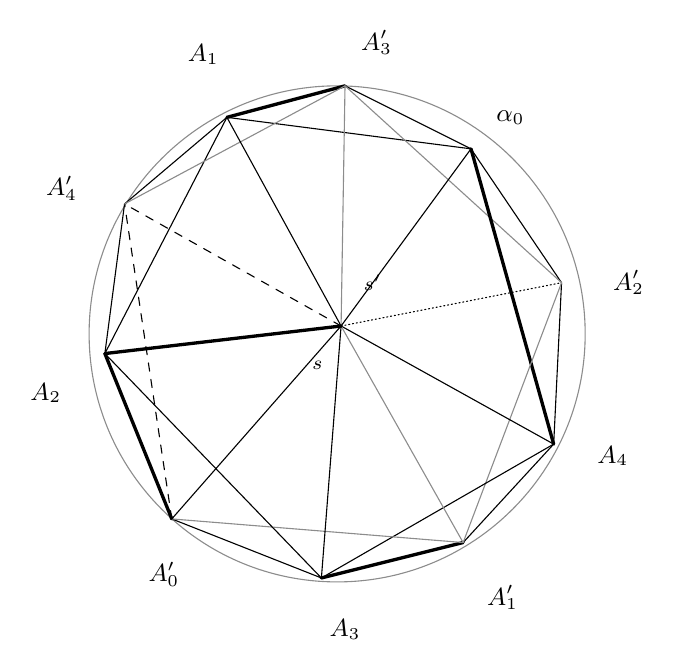
\begin{tikzpicture}[x=1mm,y=1mm,line cap=round,line join=round,font=\scriptsize]
\draw[pencil] (49,-49.5) ellipse[x radius=31.5, y radius=31.5];
\draw[very thick] (35,-22) -- (50,-18);
\draw (50,-18) -- (66,-26);
\draw (66,-26) -- (77.5,-43);
\draw (77.5,-43) -- (76.5,-63.5);
\draw (76.5,-63.5) -- (65,-76);
\draw[very thick] (65,-76) -- (47,-80.5);
\draw (47,-80.5) -- (28,-73);
\draw[very thick] (28,-73) -- (19.5,-52);
\draw (19.5,-52) -- (22,-33);
\draw (22,-33) -- (35,-22);
\draw (35,-22) -- (66,-26);
\draw[pencil] (50,-18) -- (77.5,-43);
\draw[very thick] (66,-26) -- (76.5,-63.5);
\draw[pencil] (77.5,-43) -- (65,-76);
\draw (76.5,-63.5) -- (47,-80.5);
\draw[pencil] (65,-76) -- (28,-73);
\draw (47,-80.5) -- (19.5,-52);
\draw[dashed] (28,-73) -- (22,-33);
\draw (19.5,-52) -- (35,-22);
\draw[pencil] (22,-33) -- (50,-18);
\draw (49.5,-48.5) -- (35,-22);
\draw[pencil] (49.5,-48.5) -- (50,-18);
\draw (49.5,-48.5) -- (66,-26);
\draw[densely dotted] (49.5,-48.5) -- (77.5,-43);
\draw (49.5,-48.5) -- (76.5,-63.5);
\draw[pencil] (49.5,-48.5) -- (65,-76);
\draw (49.5,-48.5) -- (47,-80.5);
\draw (49.5,-48.5) -- (28,-73);
\draw[very thick] (49.5,-48.5) -- (19.5,-52);
\draw[dashed] (49.5,-48.5) -- (22,-33);
\node[inner sep=1pt] at (32,-14) {\small $A_1$};
\node[inner sep=1pt] at (54,-12.5) {\small $A'_3$};
\node[inner sep=1pt] at (71,-22) {\small $\alpha_0$};
\node[inner sep=1pt] at (86,-43) {\small $A'_2$};
\node[inner sep=1pt] at (84,-65) {\small $A_4$};
\node[inner sep=1pt] at (70,-83) {\small $A'_1$};
\node[inner sep=1pt] at (50,-87) {\small $A_3$};
\node[inner sep=1pt] at (27,-80) {\small $A'_0$};
\node[inner sep=1pt] at (12,-57) {\small $A_2$};
\node[inner sep=1pt] at (14,-31) {\small $A'_4$};
\node[inner sep=1pt] at (53.5,-43) {\scriptsize $s'$};
\node[inner sep=1pt] at (46.5,-53.5) {\scriptsize $s$};
\end{tikzpicture}
\end{document}
